\section{Ewald selection and detector profiles}
\label{sec:si_detector_profiles}

The Ewald condition selects points from the oriented reciprocal rods. Their intensity is transformed to detector coordinates before a finite integration region defines a measured or calculated profile. This is the technical counterpart of the main-text Ewald-to-detector construction.

\subsection{Forward Ewald-surface chart and sequential Jacobians}
\label{subsec:si_ewald_surface_chart}

The local Ewald chart below connects the structural density per $dL$ to density per Ewald-surface area. The detector Jacobian then expresses that density per detector-coordinate area.

For one rod, source state, and crystallite orientation, the rotated reciprocal rod is linear in the intrinsic coordinate $L$,
\begin{equation}
  \mathbf Q_{hk}(\alpha,\beta,L)
  =\mathbf q_{hk}(\alpha,\beta)
  +L\,\mathbf d_{hk}(\alpha,\beta),
  \qquad
  \mathbf q_{hk}=\mathbf Q_{hk}(\alpha,\beta,0),
  \qquad
  \mathbf d_{hk}=\frac{\partial\mathbf Q_{hk}}{\partial L}.
  \label{eq:si_oriented_rod_affine_L}
\end{equation}
Here $\mathbf q_{hk}$ is the rotated basal offset and $\mathbf d_{hk}$ is the rod tangent per unit $L$. Let $\mathbf k'_{i,s}$ be the real internal phase wavevector and $K_s=|\mathbf k'_{i,s}|$. Squaring the elastic condition gives
\begin{equation}
  \widetilde g_{hk,s}(\alpha,\beta,L)
  =\left|\mathbf k'_{i,s}+\mathbf q_{hk}+L\mathbf d_{hk}\right|^2-K_s^2
  =A_E L^2+B_E L+C_E,
  \label{eq:si_ewald_quadratic}
\end{equation}
with
\begin{equation}
  A_E=\mathbf d_{hk}\cdot\mathbf d_{hk},
  \qquad
  B_E=2\mathbf d_{hk}\cdot\left(\mathbf k'_{i,s}+\mathbf q_{hk}\right),
  \qquad
  C_E=\left|\mathbf k'_{i,s}+\mathbf q_{hk}\right|^2-K_s^2.
  \label{eq:si_ewald_quadratic_coefficients}
\end{equation}
For discriminant $\Delta_E=B_E^2-4A_EC_E>0$, the regular Ewald branches are
\begin{equation}
  L_{hk,j,s}(\alpha,\beta)
  =\frac{-B_E\pm\sqrt{\Delta_E}}{2A_E},
  \qquad
  \mathbf Q^{E}_{hk,j,s}(\alpha,\beta)
  =\mathbf Q_{hk}\!\left[\alpha,\beta,L_{hk,j,s}(\alpha,\beta)\right].
  \label{eq:si_ewald_surface_chart}
\end{equation}
A negative discriminant means that the oriented rod misses the Ewald sphere, zero gives tangency, and a positive discriminant gives two algebraic branches. At tangency, the regular-root Jacobian is singular and the finite-region limit needs separate treatment. Equation~\eqref{eq:si_ewald_surface_chart} makes $(\alpha,\beta)$ the independent coordinates of a local two-dimensional Ewald-surface patch, while $L$ is the dependent coordinate selected by elasticity.

For derivatives of the surface chart it is convenient to use the unsquared residual
\begin{equation}
  g_{hk,s}(\alpha,\beta,L)
  =\left|\mathbf k'_{i,s}+\mathbf Q_{hk}(\alpha,\beta,L)\right|-K_s.
  \label{eq:si_ewald_unsquared_residual}
\end{equation}
For a fixed rod and source state, write $L_j=L_{hk,j,s}$ and suppress the same indices on $\mathbf Q^E$ and $J_E$. On a regular branch, implicit differentiation gives
\begin{equation}
  \frac{\partial L_j}{\partial\mu}
  =-\frac{\partial_\mu g_{hk,s}}{\partial_L g_{hk,s}},
  \qquad
  \frac{\partial\mathbf Q^E}{\partial\mu}
  =\frac{\partial\mathbf Q}{\partial\mu}
  +\frac{\partial\mathbf Q}{\partial L}
   \frac{\partial L_j}{\partial\mu},
  \qquad \mu\in\{\alpha,\beta\}.
  \label{eq:si_ewald_chart_tangents}
\end{equation}
The physical surface element is therefore
\begin{equation}
  dA_Q
  =\left|
  \frac{\partial\mathbf Q^E}{\partial\alpha}
  \times
  \frac{\partial\mathbf Q^E}{\partial\beta}
  \right|d\alpha\,d\beta
  =J_EJ_{\mathrm{vol},hk}\,d\alpha\,d\beta,
  \label{eq:si_ewald_surface_area_chart}
\end{equation}
with the real internal exit vector $\mathbf k'_{f,s}=\mathbf k'_{i,s}+\mathbf Q^E$ and Jacobians
\begin{equation}
  J_{\mathrm{vol},hk}
  =\left|
  \det\!\left[
  \partial_\alpha\mathbf Q_{hk},
  \partial_\beta\mathbf Q_{hk},
  \partial_L\mathbf Q_{hk}
  \right]
  \right|,
  \qquad
  J_E
  =\frac{1}{|\partial_L g_{hk,s}|}
  =\frac{K_s}{|\mathbf k'_{f,s}\cdot\mathbf d_{hk}|}.
  \label{eq:si_ewald_and_volume_jacobians}
\end{equation}
The optical imaginary wavevector component controls attenuation, while the real phase vectors define the Ewald sphere. The measure formulation keeps the four objects used in the main text separate: $S_{hk}(L,\lambda_s)$ is the structural rod intensity, $\mathbf Q_{hk}(\alpha,\beta,L)$ is the location map, $p_m(\alpha,\beta)$ is the orientation weight, and $J_{\mathrm{vol},hk}$ is the geometric change of measure. The pre-Ewald intensity measure is
\begin{equation}
  dI_{hk,s}^{\mathrm{pre}}
  =p_m(\alpha,\beta)S_{hk}(L,\lambda_s)
   \,d\alpha\,d\beta\,dL.
  \label{eq:si_pre_ewald_measure}
\end{equation}
Restricting this measure to the regular roots gives
\begin{equation}
  dI_{hk,j,s}^{E}
  =p_m(\alpha,\beta)S_{hk}(L_j,\lambda_s)
   J_E\,d\alpha\,d\beta.
  \label{eq:si_ewald_selected_measure}
\end{equation}
Dividing Eq.~\eqref{eq:si_ewald_selected_measure} by Eq.~\eqref{eq:si_ewald_surface_area_chart} cancels the line--sphere factor. Including the combined weight $W_{hk,j,s}$ then gives the physical Ewald-surface density
\begin{equation}
  \rho_{Q,s}^{E}(\mathbf Q)
  =\sum_{\substack{(h,k),j,\alpha,\beta\\
  \mathbf Q^{E}_{hk,j,s}(\alpha,\beta)=\mathbf Q}}
  W_{hk,j,s}
  \frac{p_m(\alpha,\beta)S_{hk}(L_j,\lambda_s)}
       {J_{\mathrm{vol},hk}}.
  \label{eq:si_ewald_surface_density_explicit}
\end{equation}
Here $W_{hk,j,s}$ includes the individual-rod population $P_{hk}$ and the source-dependent optical factors; each factor enters once. The sum includes all compatible rods, root branches and orientations. The source weight $w_s$ is applied separately when the detector images are accumulated. All branch-dependent factors are evaluated at $L=L_{hk,j,s}$. Thus $J_E$ enters the intermediate restricted measure and cancels when that measure is divided by the Ewald-surface area. The reciprocal-volume factor remains because it converts the original $(\alpha,\beta,L)$ measure into physical reciprocal-space density.

The notation $J_{\mathrm{det},s}$ is the detector Jacobian used in the main text. For continuous detector coordinates $(c_D,r_D)$, let $\mathbf Q_s(c_D,r_D)$ be the internal momentum transfer selected by that detector point and source state. Define
\begin{equation}
  J_{\mathrm{det},s}
  =\left|
  \frac{\partial\mathbf Q_s}{\partial c_D}
  \times
  \frac{\partial\mathbf Q_s}{\partial r_D}
  \right|,
  \qquad
  dA_Q=J_{\mathrm{det},s}\,dc_D\,dr_D.
  \label{eq:si_detector_surface_jacobian}
\end{equation}
The source-resolved detector-coordinate density is then
\begin{equation}
  I_{\mathrm{det},s}(c_D,r_D)
  =\sum_{\mathrm{compatible}}
  W_{hk,j,s}
  p_m(\alpha,\beta)S_{hk}(L,\lambda_s)
  \frac{J_{\mathrm{det},s}}{J_{\mathrm{vol},hk}},
  \label{eq:si_detector_density_sequential_jacobians}
\end{equation}
and the final detector density and mass $I_p$ integrated over detector pixel $p$ are
\begin{equation}
  I_{\mathrm{det}}(c_D,r_D)=\sum_s w_sI_{\mathrm{det},s}(c_D,r_D),
  \qquad
  I_p=\int_{\mathrm{pixel}\;p}I_{\mathrm{det}}(c_D,r_D)\,dc_D\,dr_D.
  \label{eq:si_source_sum_and_pixel_mass}
\end{equation}
Equation~\eqref{eq:si_detector_density_sequential_jacobians} shows the sequential change of measure directly: the reciprocal-volume Jacobian enters first and the detector-coordinate Jacobian enters second, leaving the net geometric factor $J_{\mathrm{det},s}/J_{\mathrm{vol},hk}$. The detector factor contains the pixel solid angle, detector pose and distance, source-point parallax, and the area change associated with exit refraction. An additional independent solid-angle correction would count this geometric factor twice.

Finally, the powder-cylinder factor $1/(2\pi Q_R)$ and the full determinant $J_{\mathrm{vol},hk}$ are two stages of the same azimuthal change of measure. The former expresses the density per cylinder area after distributing a rod uniformly in $\beta$. In the direct pushforward from $d\alpha\,d\beta\,dL$ to $d^3Q$, the same $\beta$-arc-length geometry is already contained in $J_{\mathrm{vol},hk}$. The determinant therefore accounts for this circumference contribution exactly once.

\subsection{Axial root and detector-coordinate evaluation}

For a fixed source state, suppress $s$ on the incident vector. The axial rod passes through the reciprocal origin. For its rotated unit direction $\hat{\mathbf d}$, write $\mathbf Q(q_z)=q_z\hat{\mathbf d}$. The elastic condition becomes
\begin{equation}
|\mathbf k'_i+q_z\hat{\mathbf d}|^2=|\mathbf k'_i|^2,
\qquad q_z(2\mathbf k'_i\cdot\hat{\mathbf d}+q_z)=0.
\label{eq:si_axial_ewald_roots}
\end{equation}
The root $q_z=0$ is the direct-beam point. The nonzero kinematic root is $q_z=-2\mathbf k'_i\cdot\hat{\mathbf d}$, with $L=q_z/|\mathbf c^*|$. For a nonunit direction $\mathbf d$ and coordinate $v$ in $\mathbf Q=v\mathbf d$, the second root is $v=-2\mathbf k'_i\cdot\mathbf d/(\mathbf d\cdot\mathbf d)$.

The forward roots provide a geometric construction. In detector-coordinate evaluation, a detector point fixes the outgoing air ray, exit refraction fixes the internal phase vector, and their difference supplies $\mathbf Q_s$. The inverse reciprocal map then returns all compatible rods, orientations and intrinsic $L$ values. Both descriptions use the density in Eq.~\eqref{eq:si_detector_density_sequential_jacobians}. Since $dA_Q=K_s^2d\Omega$, density per internal outgoing solid angle is $K_s^2\rho_{Q,s}^E$.

\subsection{Finite integration and projected coordinates}
\label{subsec:si_projection_uncertainty}

Here $d\Omega$ is an element of internal outgoing solid angle. The detector image remains the primary data object. The $2\theta$--$\phi_f$ representation is an overlap-weighted remapping used to evaluate fixed-$r$ or fixed-$Q_R$ trajectory masks and projected $Q_z$ or $L_{\mathrm{proj}}$ profiles. Its statistical information comes from the original detector image. The same remapping, masks, and profile extraction are applied to measured and calculated detector images.

The caked image is constructed with a sparse detector-to-cake operator
\begin{equation}
\mathbf M_{\mathrm{cake}}\in \mathbb{R}^{N_{\mathrm{bin}}\times N_{\mathrm{pix}}},
\end{equation}
where $N_{\mathrm{pix}}$ is the number of detector pixels, $N_{\mathrm{bin}}$ is the number of caked bins, and $M^{\mathrm{cake}}_{bp}$ is the fractional overlap weight from detector pixel $p$ into caked bin $b$. For detector signal $s_p$ and normalization $n_p$, define accumulated caked-bin signal $S_b$, normalization $N_b$ and normalized intensity $I_b$:
\begin{equation}
S_b=\sum_p M^{\mathrm{cake}}_{bp}s_p,
\qquad
N_b=\sum_p M^{\mathrm{cake}}_{bp}n_p,
\qquad
I_b=\frac{S_b}{N_b},
\end{equation}
for bins with $N_b>0$. Signal and normalization are therefore accumulated before division. This prevents a projected profile from becoming a sum of already normalized pixels and keeps the observable tied to the detector-space calibration.

For each remapped bin, the calibrated detector and sample geometry define a scattering vector $\mathbf Q$. The coordinates used to label selected trajectories are
\begin{equation}
\mathbf Q_{\parallel}
=\mathbf Q-(\mathbf Q\cdot\hat{\mathbf n})\hat{\mathbf n},
\qquad
Q_R=|\mathbf Q_{\parallel}|,
\qquad
Q_z=\mathbf Q\cdot \hat{\mathbf n},
\qquad
L_{\mathrm{proj}}=\frac{Q_z}{|\mathbf c^{*}|}=\frac{Q_z c}{2\pi},
\end{equation}
where $\hat{\mathbf n}$ is the film normal and $\mathbf Q_{\parallel}$ is the component within its plane. For a hexagonal basal plane, the dimensionless radial-family index associated with $(h,k)$ is $r\equiv h^2+hk+k^2$. The index $r$ labels a discrete family. Its radius is $Q_R(r)$, and the explicit sum over individual $(h,k)$ members accounts for multiplicity. For target radius $Q_{R,0}$, radial half-width $\Delta Q_R$ and accepted projected limits $Q_{z,\min}$ and $Q_{z,\max}$, a fixed-$Q_R$ or fixed-$r$ family is retained when
\begin{equation}
|Q_R-Q_{R,0}|\le \Delta Q_R,
\qquad
Q_{z,\min}\le Q_z\le Q_{z,\max}.
\end{equation}
This region is simple in the physical $Q_R$--$Q_z$ description but appears curved in the displayed $2\theta$--$\phi_f$ map because the coordinate transformation is nonlinear. The coordinate projection fully accounts for the curved shape.

For a selected profile-bin index $\nu$, let $\mu_{\nu b}$ be the mask or interpolation weight that assigns caked bin $b$ to that profile point. Write $S_\nu=\sum_b\mu_{\nu b}S_b$ and $N_\nu=\sum_b\mu_{\nu b}N_b$ for its accumulated signal and normalization. The profile is
\begin{equation}
I_{\nu}^{\mathrm{ROI}}=\frac{S_\nu}{N_\nu}=
\frac{\sum_b \mu_{\nu b}S_b}
     {\sum_b \mu_{\nu b}N_b}
=
\frac{\sum_p a_{\nu p}s_p}
     {\sum_p a_{\nu p}n_p},
\qquad
 a_{\nu p}=\sum_b \mu_{\nu b}M^{\mathrm{cake}}_{bp}.
\label{eq:si_profile_average}
\end{equation}
Each point in the plotted profile is therefore an average over a finite detector-space band. Its coordinate may be labeled by $Q_z$ or $L_{\mathrm{proj}}$, and the point represents a finite-bin projection over the accepted reciprocal-space interval.

Intrinsic $L$ belongs to the crystallite-frame rod. The nominal detector projection $L_{\mathrm{proj}}$ uses the mean film normal and the declared reference beam. A fixed detector point generally has a different source-resolved $\mathbf Q_s$ for each incident state. Source-resolved physical reciprocal maps and nominal measured-image displays are therefore distinguished. The same nominal display map is applied to measured and calculated detector images.

\begin{figure}[!htbp]
\centering
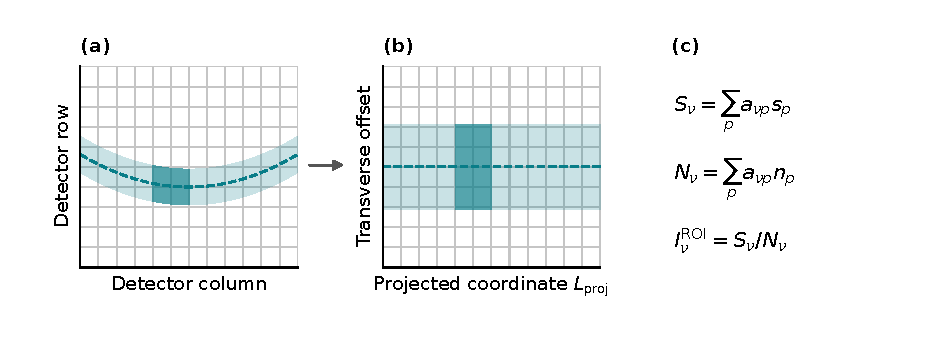
\includegraphics[width=\linewidth]{figures/profile_construction_guide.pdf}
\caption{Construction of a finite-region detector profile. (a) A curved integration band crosses native detector pixels. Teal shading marks accepted area, and the darker segment marks one selected profile interval. (b) A coordinate transformation straightens the band into a strip, where the same darker interval is retained. Gray grid lines show pixel or bin boundaries, and the dashed line marks the trajectory center. (c) Detector signal and normalization pass through the same overlap and mask weights before their accumulated values are divided. The equations define an average over the accepted area.}
\label{fig:si_profile_construction}
\end{figure}

Coordinate and intensity uncertainty are derived in Sec.~\ref{subsec:si_uncertainty}. The finite integration in Fig.~\ref{fig:si_profile_construction} is common to the ordered comparisons in Sec.~\ref{sec:si_ordered_comparisons} and the selected PbI$_2$ profiles in Sec.~\ref{sec:si_pbi2_transition}.
